%% LyX 2.1.4 created this file.  For more info, see http://www.lyx.org/.
%% Do not edit unless you really know what you are doing.
\documentclass[a4paper,english,british]{article}
\usepackage[T1]{fontenc}
\usepackage[latin9]{inputenc}
\usepackage{babel}
\usepackage{amsmath}
\usepackage{amsthm}
\usepackage{amssymb}
\usepackage{graphicx}
\usepackage[numbers]{natbib}
\usepackage[unicode=true]
 {hyperref}

\makeatletter

%%%%%%%%%%%%%%%%%%%%%%%%%%%%%% LyX specific LaTeX commands.
\pdfpageheight\paperheight
\pdfpagewidth\paperwidth


%%%%%%%%%%%%%%%%%%%%%%%%%%%%%% Textclass specific LaTeX commands.
\theoremstyle{plain}
\newtheorem{thm}{\protect\theoremname}[section]
  \theoremstyle{plain}
  \newtheorem{lem}[thm]{\protect\lemmaname}
  \theoremstyle{plain}
  \newtheorem{prop}[thm]{\protect\propositionname}

%%%%%%%%%%%%%%%%%%%%%%%%%%%%%% User specified LaTeX commands.
% from the icml 2016 example tex file
\usepackage{times}
\usepackage{algorithm}
\usepackage{algorithmic}
\usepackage{hyperref}
%\newcommand{\theHalgorithm}{\arabic{algorithm}}
\usepackage[accepted]{icml2016} 
\usepackage{placeins}

%\usepackage[accepted]{icml2016}


\newcommand{\heiko}[1]{   {\bf \color{blue}{HS: #1}}  }
\newcommand{\kacper}[1]{   {\bf \color{red}{K: #1}}  }
\newcommand{\arthur}[1]{   {\bf \color{magenta}{AG: #1}}  }

%\newcommand{\heiko}[1]{}

\makeatother

  \addto\captionsbritish{\renewcommand{\lemmaname}{Lemma}}
  \addto\captionsbritish{\renewcommand{\propositionname}{Proposition}}
  \addto\captionsbritish{\renewcommand{\theoremname}{Theorem}}
  \addto\captionsenglish{\renewcommand{\lemmaname}{Lemma}}
  \addto\captionsenglish{\renewcommand{\propositionname}{Proposition}}
  \addto\captionsenglish{\renewcommand{\theoremname}{Theorem}}
  \providecommand{\lemmaname}{Lemma}
  \providecommand{\propositionname}{Proposition}
\providecommand{\theoremname}{Theorem}

\begin{document}
\twocolumn[ \icmltitle{A Kernel Test of Goodness of Fit}
% It is OKAY to include author information, even for blind
% submissions: the style file will automatically remove it for you
% unless you've provided the [accepted] option to the icml2015
% package.
\icmlauthor{Kacper Chwialkowski$^*$}{kacper.chwialkowski@gmail.com}
\icmlauthor{Heiko Strathmann$^*$}{heiko.strathmann@gmail.com}
\icmlauthor{Arthur Gretton}{arthur.gretton@gmail.com}
\icmladdress{Gatsby Unit, University College London, United Kingdom}
% You may provide any keywords that you 
% find helpful for describing your paper; these are used to populate
% the "keywords" metadata in the PDF but will not be shown in the document
\icmlkeywords{kernel methods, goodness-of-fit, Stein's method, statistical testing}
\vskip 0.3in ]

\begin{abstract}
We propose a nonparametric statistical test for goodness-of-fit: given
a set of samples, the test determines how likely it is that these
were generated from a target density function. The measure of goodness-of-fit
is a divergence constructed via Stein's method using functions from
a Reproducing Kernel Hilbert Space. Our test statistic is based on
an empirical estimate of this divergence, taking the form of a V-statistic
in terms of the log gradients of the target density and the kernel.
We derive a statistical test, both for i.i.d. and non-i.i.d. samples,
where we estimate the null distribution quantiles using a wild bootstrap
procedure. We apply our test to quantifying convergence of approximate
Markov Chain Monte Carlo methods, statistical model criticism, and
evaluating quality of fit vs model complexity in nonparametric density
estimation.
\end{abstract}
\selectlanguage{english}%
\global\long\def\ev{\mathbb{E}}


\selectlanguage{british}%

\section{Introduction}

Statistical tests of goodness-of-fit are a fundamental tool in statistical
analysis, dating back to the test of Kolmogorov and Smirnov \citep{Kolmogorov33,Smirnov48}.
Given a set of samples $\{Z_{i}\}_{i=1}^{n}$ with distribution $Z_{i}\sim q$,
our interest is in whether $q$ matches some reference or target distribution
$p$\foreignlanguage{english}{, which we assume to be only known up
to the normalisation constant. Recently, in the multivariate setting,
}\citet{gorham2015measuring} proposed an elegant measure of sample
quality with respect to a target. This measure is a maximum discrepancy
between empirical sample expectations and target expectations over
a large class of test functions, constructed so as to have zero expectation
over the target distribution by use of a Stein operator. This operator
depends only on the derivative of the $\log q$: thus, the approach
can be applied very generally, as it does not require closed-form
integrals over the target distribution (or numerical approximations
of such integrals). By contrast, many earlier discrepancy measures
require integrals with respect to the target (see below for a review).
This is problematic if the intention is to perform benchmarks for
assessing Markov Chain Monte Carlo, since these integrals will certainly
not be known to the practitioner.

A challenge in applying the approach of \citeauthor{gorham2015measuring}
is the complexity of the function class used, which results from applying
the Stein operator to the bounded Lipschitz functions.\footnote{The bounded Lipschitz functions give rise to the Wasserstein integral
probability metric. By contrast, the Kolmogorov-Smirnov test uses
functions of bounded variation 1 \citep{Mueller97}. Multivariate
generalisations of the K-S test exist, however the computational cost
of a consistent test rapidly becomes prohibitive with increasing dimension
\citep{Justel1997251}.} Thus, their sample quality measure requires solving an expensive
linear program that arises from a complicated construction of graph
Stein discrepancies and geometric spanners. Their metric furthermore
requires access to nontrivial lower bounds that, despite being provided
for log-concave densities, are a largely open problem otherwise, in
particular for multivariate cases.

An important application of a goodness-of-fit measure is in statistical
testing, where it is desired to determine whether the empirical discrepancy
measure is large enough to reject the null hypothesis (that the sample
arises from the target distribution). One approach is to establish
the asymptotic behaviour of the test statistic, and to set a test
threshold at a large quantile of the asymptotic distribution. The
asymptotic behaviour of the Wasserstein-based Stein discrepancy remains
a challenging open problem, due to the complexity of the function
class used. It is not clear how one would compute p-values for this
statistic, or determine when the goodness of fit test would allow
us to accept the null hypothesis (at the user-specified test level).

The key contribution of this work is to define a statistical test
of goodness-of-fit, based on a Stein discrepancy computed in a Reproducing
Kernel Hilbert Space (RKHS).  To construct our test statistic, we
use a function class defined by applying the Stein operator to a chosen
space of RKHS functions, as proposed by \citep{OatGirCho15}.\footnote{\citeauthor{OatGirCho15} addressed the problem variance reduction
in Monte Carlo integration, using the Stein operator to avoid bias. } Our measure of goodness of fit is the largest discrepancy over this
space of functions between empirical sample expectations and target
expectations (the latter being zero, due to the effect of the Stein
operator). The approach is a natural extension to goodness-of-fit
testing of the earlier two-sample tests \citep{gretton2012kernel}
and independence tests \citep{gretton_kernel_2008} based on the maximum
mean discrepancy, which is an integral probability metric. As with
these earlier tests, our statistic is a simple V-statistic, and can
be computed in closed form and in quadratic time; moreover, it is
an unbiased estimate of the corresponding population discrepancy.
As with all Stein-based discrepancies, only the gradient of the log-density
of the target density is needed; we do not require integrals with
respect to the target density -- including the normalisation constant.
Given that our test statistic is a V-statistic, we may make use of
the extensive literature on asymptotics of V-statistics to formulate
a hypothesis test \citep{serfling80,leucht_dependent_2013}.  We
are able to provide statistical tests for both uncorrelated and correlated
samples, where the latter is essential if the test is to be used in
assessing the quality of output of an MCMC procedure.  An identical
test was obtained simultaneously in independent work by \citet{LiuLeeJor16},
for uncorrelated samples.

Several alternative approaches exist in the statistics literature
to goodness-of-fit testing. A first strategy is to partition the space,
and to conduct the test on a histogram estimate of the distribution
\citep{Bar89,Beirlant2,Gyorfi,GyVa02}.\foreignlanguage{english}{
Such space partitioning approaches can have attractive theoretical
properties (e.g. distribution-free test thresholds) and work well
in low dimensions, however they are much less powerful than alternatives
once the dimensionality increases \citep{GreGyo10}.} A second popular
approach has been to use the smoothed $L_{2}$ distance between the
empirical characteristic function of the sample, and the characteristic
function of the target density. This dates back to the test of Gaussianity
of \citet{BaringhausHenze88}, who used a squared exponential smoothing
function (see Eq. 2.1 in their paper). For this choice of smoothing
function, their statistic is identical to the maximum mean discrepancy
(MMD) with the squared exponential kernel, which can be shown using
the Bochner representation of the kernel (compare with \citealt[Corollary 4]{SriGreFukLanetal10}).
It is essential in this case that the target distribution be Gaussian,
since the convolution with the kernel (or in the Fourier domain, the
smoothing function) must be available in closed form. An $L_{2}$
distance between Parzen window estimates can also be used  \citep{BowFos93},
giving the same expression again, although the optimal choice of bandwidth
for consistent Parzen window estimates may not be a good choice for
testing \citep{AndHalTit94}. A different smoothing scheme in the
frequency domain results in an energy distance statistic \citep[this likewise being an MMD with a particular choice of kernel; see ][]{SejSriGreFuk13},
which can be used in a test of normality \citep{SzeRiz05}. The key
point is that the required integrals are again computable in closed
form for the Gaussian, although the reasoning may be extended to certain
other families of interest, e.g. \citep{Rizzo09}. The requirement
of computing closed-form integrals with respect to the test distribution
severely restricts this testing strategy. Finally, a problem related
to goodness-of-fit testing is that of model criticism \citep{lloyd2015statistical}.
In this setting, samples generated from a fitted model are compared
via the maximum mean discrepancy with samples used to train the model,
such that a small MMD indicates a good fit. There are two limitation
to the method: first, it requires samples from the model (which might
not be easy if this requires a complex MCMC sampler); second, the
choice of number of samples from the model is not obvious, since too
few samples cause a loss in test power, and too many are computationally
wasteful. Neither issue arises in our test, since we do not require
model samples.

In our experiments, a particular focus is on applying our goodness-of-fit
test to certify the output of approximate Markov Chain Monte Carlo
(MCMC) samplers \citep{Korattikara2014,Welling2011,Bardenet2014}.
These methods use modifications to Markov transition kernels that
improve mixing speed at the cost of worsening the asymptotic bias.
The bias-variance trade-off can usually be tuned with parameters of
the sampling algorithms. It is therefore important to test whether
for a particular parameter setting and run-time, the samples are of
the desired quality. This question cannot be answered with classical
MCMC convergence statistics, such as the widely used potential scale
reduction factor (R-factor) \citep{gelman1992inference} or the effective
sample size, since these assume that the Markov chain reaches its
equilibrium distribution. By contrast, our test exactly quantifies
the asymptotic bias of approximate MCMC. 

See \href{https://github.com/karlnapf/kernel_goodness_of_fit}{https://github.com/karlnapf/kernel\_{}goodness\_{}of\_{}fit} for code.


\paragraph{Paper outline}

We begin our presentation in the section \ref{sec:A-Kernel-Goodness-of-fit}
with a high-level construction of the RKHS-based Stein discrepancy
and associated statistical test. In Section \ref{sec:Details}, we
provide additional details and prove the main results. Section \ref{sec:experiment}
contains experimental illustrations on synthetic examples, statistical
model criticism, bias-variance trade-offs in approximate MCMC, and
convergence in non-parametric density estimation.

\selectlanguage{english}%

\section{Test Definition: Statistic and Threshold\label{sec:A-Kernel-Goodness-of-fit}}

We begin with a high-level construction of our divergence discrepancy
and the statistical test. While this section aims to communicate the
main ideas, we provide details and proofs in Section \ref{sec:Details}.


\subsection{Stein Operator in RKHS}

Our goal is to write the maximum discrepancy between target distribution
$p$ and observed sample distribution $q$ in a RKHS. Denote by ${\cal F}$
the RKHS of real-valued functions on $\mathbb{R}^{d}$ with reproducing
kernel $k$, and by ${\cal F}^{d}$ the product RKHS consisting of
elements $f:=(f_{1},\dots,f_{d})$ with $f_{i}\in{\cal F}$, and with
a standard inner product $\left\langle f,g\right\rangle _{\mathcal{F}^{d}}=\sum_{i=1}^{d}\left\langle f_{i},g_{i}\right\rangle _{\mathcal{F}}$.
Similarly to \citet{stein1972,gorham2015measuring,OatGirCho15}, we
begin by defining a Stein operator $T$ acting on $f\in\mathcal{F}^{d}$
\[
Tf:=\sum_{i=1}^{d}\left(\frac{\partial\log p(x)}{\partial x_{i}}f_{i}(x)+\frac{\partial f_{i}(x)}{\partial x_{i}}\right).
\]
Suppose a random variable $Z$ is distributed according to a measure\footnote{\selectlanguage{british}%
Throughout the article, all occurrences of $Z$, e.g. $Z',Z_{i},Z_{\heartsuit}$,
are understood to be distributed according to $q$.\selectlanguage{english}%
} $q$ and $X$ is distributed according to the target measure $p$.
As we will see, the operator can be expressed by defining a function
that depends on gradients of the log-density and the kernel, 
\begin{equation}
\xi(x,\cdot):=\left[\nabla\log p(x)k(x,\cdot)+\nabla k(x,\cdot)\right],\label{eq:xi}
\end{equation}
whose inner product with $f$ gives exactly the expected value of
the Stein operator 
\[
\ev Tf(Z)=\langle f,\ev\xi(Z)\rangle_{{\cal F}^{d}}=\sum_{i=1}^{d}\langle f_{i},\ev\xi_{i}(Z)\rangle_{{\cal F}},
\]
c.f. Lemma \ref{lem:SteinIsInner}. For $X$ from the target measure,
we have $\ev(Tf)(X)=0$, which can be seen using integration by parts,
c.f. Lemma \ref{lem:easy} in the supplement. We can now define a
Stein discrepancy and express it in the RKHS,
\begin{align*}
S(Z) & :=\sup_{\Vert f\Vert<1}\ev(Tf)(Z)-\ev(Tf)(X)\\
 & =\sup_{\Vert f\Vert<1}\langle f,\ev\xi(Z)-\ev\xi(X)\rangle_{{\cal F}^{d}}\\
 & =\sup_{\Vert f\Vert<1}\langle f,\ev\xi(Z)\rangle_{{\cal F}^{d}}\\
 & =\|\ev\xi(Z)\|_{{\cal F}^{d}},
\end{align*}
c.f. Lemma \ref{lem:discprepancy_maximised_by_norm}. This makes it
clear why $\ev(Tf)(X)=0$ is a desirable property: we can compute
$S(Z)$ by computing $\|\ev\xi(Z)\|$, without the need to access
$X$ in the form of samples from $p$. We arrive at our first main
result, which states that the above discrepancy can be used to distinguish
two distributions $p,q\in{\cal P}$.
\begin{thm}
\label{theorem_discrepancy_is_metric} Let $q,p\in\mathcal{P}$ where
the derivatives of elements of $\mathcal{P}$ satisfy assumption (ii)
in Section \ref{sec:details_kernel_stein}, and let $Z\sim q$. Let
the RKHS $\mathcal{F}$ satisfy properties (iii) and (v) in Section
\ref{sec:details_kernel_stein}, which include the requirement that
$\mathcal{F}$ be cc-universal \citep[Definition 4.1]{carmeli2010vector}.
Then $S(Z)=0$ if and only if $p=q$. 
\end{thm}
\selectlanguage{british}%
Section \ref{sec:details_kernel_stein} contains the formal statements
of the assumptions on ${\cal P}$ and $\mathcal{F}$, and a proof.
The following theorem gives a simple closed form expression.
\selectlanguage{english}%
\begin{thm}
\label{th:closed_form_discrepancy} Let 
\begin{align*}
h(x,y) & :=\nabla\log p(x)^{\top}\nabla\log p(y)k(x,y)\\
 & \quad+\nabla\log p(y)^{\top}\nabla_{x}k(x,y)\\
 & \quad+\nabla\log p(x){}^{\top}\nabla_{y}k(x,y)\\
 & \quad+\langle\nabla_{x}k(x,\cdot),\nabla_{y}k(\cdot,y)\rangle_{{\cal F}^{d}},
\end{align*}


where the last term can be written as a sum $\sum_{\{i=1\}}^{d}\frac{\partial k(x,y)}{\partial x_{i}\partial y_{i}}$.
The \foreignlanguage{british}{squared Stein discrepancy is} $S(Z)^{2}=\ev h(Z,Z')$.\foreignlanguage{british}{ }
\end{thm}
\selectlanguage{british}%
We now proceed with constructing an estimator for $S(Z)^{2}$, and
outline its asymptotic properties.


\subsection{Wild Bootstrap Testing}

It is straightforward to estimate the squared Stein discrepancy $S(Z)^{2}$
from samples $\{Z_{i}\}_{i=1}^{n}$: a quadratic time estimator is
a V-Statistic, and takes the form
\[
V_{n}=\frac{1}{n^{2}}\sum_{i,j=1}^{n}h(Z_{i},Z_{j}).
\]
 The asymptotic null distribution of the normalised V-Statistic $nV_{n}$,
however, has no computable closed form. Furthermore, care has to be
taken when the $Z_{i}$ exhibit correlation structure, as the null
distribution significantly changes, impacting test significance. The
wild bootstrap technique \citep{Shao2010,leucht_dependent_2013,FroLauLerRey12}
addresses both problems. First, it allows to simulate from the null
distribution to compute test thresholds. Second, it accounts for correlation
structure in the $Z_{i}$ by mimicking it with an \foreignlanguage{english}{auxiliary}
random process: a\foreignlanguage{english}{ Markov chain taking values
in $\{-1,1\}$, starting from $W_{1,n}=1$,}
\[
W_{t,n}=\mathbf{1}(U_{t}>a_{n})W_{t-1,n}-\mathbf{1}(U_{t}<a_{n})W_{t-1,n},
\]
\foreignlanguage{english}{where the $U_{t}$ are uniform i.i.d. random
variables and $a_{n}$ is the probability of $W_{t,n}$ changing sign
(for i.i.d. data we may set $a_{n}=0.5$). This leads to a bootstrapped
V-statistic }

\selectlanguage{english}%
\emph{
\[
B_{n}=\frac{1}{n^{2}}\sum_{i,j=1}^{n}W_{i,n}W_{j,n}h(Z_{i,}Z_{j}).
\]
}Proposition \ref{thm:wild_bootstrap_works}\foreignlanguage{british}{
establishes that, under the null hypothesis, $nB_{n}$} is a good
approximation of $nV_{n}$, so it is possible to approximate quantiles
of the null distribution by sampling from it. Under the alternative,
however, $V_{n}$ dominates $B_{n}$ -- resulting in almost sure rejection
of the null hypothesis.

We propose the following test\foreignlanguage{british}{ procedure
for testing the null hypothesis that the $Z_{i}$ are distributed
according to the target distribution $p$.}
\selectlanguage{british}%
\begin{itemize}
\item Calculate \foreignlanguage{english}{the test statistic $V_{n}$.}
\selectlanguage{english}%
\item Obtain wild bootstrap samples\foreignlanguage{british}{ }$\{B_{n}\}_{i=1}^{D}$
and estimate the $1-\alpha$ empirical quantile of these samples. 
\item If $V_{n}$ exceeds the quantile, reject.
\end{itemize}
\selectlanguage{english}%

\section{Proofs of the Main Results\label{sec:Details}}

We now prove the claims made in the previous Section.


\subsection{Stein Operator in RKHS}

\label{sec:details_kernel_stein}

We make the following assumptions. Let ${\cal P}$ be a family of
distributions on a real coordinate space, where its elements $p\in\mathcal{P}$
satisfy two conditions:

\begin{itemize}
	\item[(i)]  $\nabla \log p(x)$ is Lipschitz continuous.
	\item[(ii)] $\mathbb E \| \nabla \log p(Z) \|^2 \leq \infty$ for any random variable.
\end{itemize}

The kernels $k$ considered in this work satisfy

\begin{itemize}
	\item[(iii)]  $\mathbb E  \left( \frac{\partial^2 k(Z,Z)}{\partial x_i \partial x_{i+d}} \right)^2 \leq \infty$. 
	\item[(iv)] $\nabla_x k(x,y)$ is Lipschitz continuous.
    \item[(v)] $k$ is bounded, symmetric and cc-universal \citep{carmeli2010vector}.
\end{itemize}

\selectlanguage{british}%
Requirements (i) and (iv) are used in Proposition \ref{thm:wild_bootstrap_works}
regarding the wild-bootstrap procedure, (ii) and (iii) are needed
for Bocher integrability of $\xi$ in Lemma \ref{lem:BochnerInt1},
and (v) is needed in the proof of Theorem \ref{theorem_discrepancy_is_metric}.\foreignlanguage{english}{ }

\selectlanguage{english}%
We show in Lemma \ref{lem:easy} in the Appendix that the expected
value of the Stein operator is zero on the target measure.

The following lemmas are useful in proving our main results, Theorems
\ref{th:closed_form_discrepancy} and \ref{theorem_discrepancy_is_metric}.
\begin{lem}
\label{lem:WellDefined} $\xi(x,\cdot)$ (see \foreignlanguage{british}{Eq.
(\ref{eq:xi})}) is an element of the reproducing kernel Hilbert space
$\mathcal{F}^{d}$. \end{lem}
\begin{proof}
We use the proof of \citet[Corollary 4.36]{SteChr08} to see that
for all $x\in R^{d}$ each entry of $\nabla k(x,\cdot)$ belongs to
$\mathcal{F}$. $\frac{\partial\log p(x)}{\partial x_{i}}k(x,\cdot)\in\mathcal{F}$,
since $k(x,\cdot)\in\mathcal{F}$ and $\frac{\partial\log p(x)}{\partial x_{i}}$
is a scalar. 
\end{proof}
\selectlanguage{british}%
The following lemma shows that the expected value of $\xi$ is well
defined -- it is needed for establishing a link between Stein operator
$Tf$ and $\xi$.
\selectlanguage{english}%
\begin{lem}
\label{lem:BochnerInt1}For any random variable $Z$, the expected
value of $\xi(Z)$ is an element of $\mathcal{F}^{d}$ (\textup{$\xi$}
is Bochner integrable wrt the measure of $Z$). \end{lem}
\begin{proof}
It is sufficient to check that coefficients of $\xi$ are Bochner
integrable \citep[Definition A.5.20]{SteChr08}. First we check that
for any random variable $Z$, 
\[
\ev\left\Vert \frac{\partial\log p(Z)}{\partial x_{i}}k(Z,\cdot)\right\Vert _{\mathcal{F}}^{2}<C\ev\|\nabla\log p(X)\|^{2}<\infty,
\]
for some constant $C$, which follows from assumption (ii) and boundedness
of the kernel. Next we check that 
\[
\ev\left\Vert \frac{\partial k(Z,\cdot)}{\partial x}\right\Vert _{\mathcal{F}^{d}}^{2}=\ev\left(\frac{\partial^{2}k(Z,Z)}{dx_{i}dx_{i+d}}\right)^{2}<\infty,
\]
which follows from assumption (iii).
\end{proof}
\selectlanguage{british}%
We can now show that the expected value of the Stein operator can
be expressed as an inner product with an element of $\mathcal{F}^{d}$,
where this element is the expected value of $\xi$. 
\selectlanguage{english}%
\begin{lem}
\label{lem:SteinIsInner}For any random variable $Z$, the expected
value of the Stein operator coincides with the inner product of $f$
and the expected value of $\xi(Z)$, 
\begin{align*}
\ev Tf(Z)=\langle f,\ev\xi(Z)\rangle_{\mathcal{F}^{d}} & =\sum_{i=1}^{d}\langle f_{i},\ev\xi_{i}(Z)\rangle_{\mathcal{F}}.
\end{align*}
\end{lem}
\begin{proof}
We write
\begin{align*}
 & \left\langle f_{i},\ev\xi_{i}(Z)\right\rangle _{\mathcal{F}}\\
 & =\left\langle f_{i},\ev\left[\frac{\partial\log p(Z)}{\partial x_{i}}k(Z,\cdot)+\frac{\partial k(Z,\cdot)}{\partial x_{i}}\right]\right\rangle _{\mathcal{F}}\\
 & =\ev\left\langle f_{i},\frac{\partial\log p(Z)}{\partial x_{i}}k(Z,\cdot)+\frac{\partial k(Z,\cdot)}{\partial x_{i}}\right\rangle _{\mathcal{F}}\\
 & =\ev\left[\frac{\partial\log p(Z)}{\partial x_{i}}f_{i}(Z)+\frac{\partial f(Z,\cdot)}{\partial x_{i}}\right].
\end{align*}
The second equality follows from the fact that a linear operator $\langle f_{i},\cdot\rangle_{\mathcal{F}}$
can be interchanged with the Bochner integral, and the fact that $\xi$
is Bochner integrable (Lemma \ref{lem:BochnerInt1}). The last equality
is an application of the reproducing property. 
\end{proof}
From the inner product representation, we get  
\begin{lem}
\label{lem:discprepancy_maximised_by_norm}The discrepancy $S(Y,\mathcal{F},p)$
is maximized by the expected value of $\xi$, i.e. $S(Y,\mathcal{F},p)=\|\ev\xi(Y)\|$.\end{lem}
\begin{proof}
By the Lemma \foreignlanguage{british}{\ref{lem:SteinIsInner}, }$\ev Tf(Y)=\langle f,\ev\xi(Y)\rangle_{\mathcal{F}^{d}}$
and therefore, $S(Y,\mathcal{F},p)$ is maximized by $\frac{\ev\xi(Y)}{\|\ev\xi(Y)\|_{\mathcal{F}^{d}}}$.
\end{proof}
We are now ready for the proof\foreignlanguage{british}{ of the closed
form formula for }$S(Y,\mathcal{F},p)^{2}$.
\begin{proof}[Proof of Theorem \ref{th:closed_form_discrepancy}]
 We use the notation 
\begin{align*}
\nabla_{x}k(x,\cdot)=\left(\frac{\partial k(x,\cdot)}{\partial x_{1}},\cdots,\frac{\partial k(x,\cdot)}{\partial x_{d}}\right)\\
\nabla_{y}k(\cdot,y)=\left(\frac{\partial k(\cdot,y)}{\partial y_{1}},\cdots,\frac{\partial k(\cdot,y)}{\partial y_{d}}\right),
\end{align*}
giving 
\begin{align*}
 & S(X,\mathcal{F},p)^{2}=\langle\ev\xi,\ev\xi\rangle_{\mathcal{F}^{d}}\\
 & =\langle\ev\left[\nabla\log p(X)k(X,\cdot)+\nabla_{x}k(X,\cdot)\right],\\
 & \quad\quad\ev\left[\nabla\log p(X)k(X,\cdot)+\nabla_{x}k(X,\cdot)\right]\rangle_{\mathcal{F}^{d}}\\
 & =\ev\langle\nabla\log p(X)k(X,\cdot)+\nabla_{x}k(X,\cdot),\\
 & \quad\quad\quad\nabla\log p(X)k(\cdot,X')+\nabla_{y}k(\cdot,X')\rangle_{\mathcal{F}^{d}}\\
 & =\ev\nabla\log p(X)^{\top}\nabla\log p(X')k(X,X')\\
 & \quad+\ev\nabla\log p(X)\nabla_{x}k(X,X')\\
 & \quad+\ev\nabla\log p(X){}^{\top}\nabla_{y}k(X,X')\\
 & \quad+\ev\langle\nabla_{x}k(X,\cdot),\nabla_{y}k(\cdot,X')\rangle_{\mathcal{F}^{d}}.
\end{align*}

\end{proof}
\selectlanguage{british}%
Finally, we prove that \foreignlanguage{english}{the discrepancy $S$
discriminates different probability measures. }
\selectlanguage{english}%
\begin{proof}[Proof of Theorem \ref{theorem_discrepancy_is_metric}]
 If $p=q$ then $S(Y,\mathcal{F},p)$ is $0$ by Lemma (\ref{lem:easy}).
Suppose $p\neq q$, but $S(Y,\mathcal{F},p)=0$. If $S(Y,\mathcal{F},p)=0$
then $\ev\xi(Y)=0.$ For each dimension of $\ev\xi(Y)$, we add and
subtract $\log q(Y)$, 
\begin{align*}
 & \ev\left(\frac{\partial}{\partial x_{i}}\log p(Y)k(Y,\cdot)+\frac{\partial}{\partial x_{i}}k(Y,\cdot)\right)\\
 & =\ev\left(\frac{\partial}{\partial x_{i}}(\log q(Y))k(Y,\cdot)+\frac{\partial}{\partial x_{i}}k(Y,\cdot)\right)\\
 & \quad+\ev\left(\frac{\partial}{\partial x_{i}}(\log p(Y)-\log q(Y))k(Y,\cdot)\right).
\end{align*}
We have used Lemma \ref{lem:easy} to see that 
\[
\ev\left(\frac{\partial}{\partial x_{i}}(\log q(Y))k(Y,\cdot)+\frac{\partial}{\partial x_{i}}k(Y,\cdot)\right)=0.
\]
We \foreignlanguage{british}{recognise} that the expected value of
$\frac{\partial}{\partial x_{i}}(\log p(Y)-\log q(Y))k(Y,\cdot)$
is the mean embedding of a function $g(y)=\frac{\partial}{\partial x_{i}}\left(\log\frac{p(y)}{q(y)}\right)$
with respect to the measure $q$. By assumption (ii) function $g$
is square integrable, $\ev(\frac{\partial}{\partial x_{i}}\log p(Y))^{2}\leq\infty$
and $\ev(\frac{\partial}{\partial x_{i}}\log q(Y))^{2}\leq\infty$
. Therefore, since the kernel $k$ is cc-universal, by \citet[ Theorem 4.4 c]{carmeli2010vector}
this embedding is zero if and only if $g=0$, which implies that 
\[
\nabla\log\frac{p(y)}{q(y)}=(0,\cdots,0).
\]
A constant vector field of derivatives can only be generated by a
constant function, so $\log\frac{p(y)}{q(y)}=C$, for some $C$, which
implies that $p(y)=e^{C}q(y)$. Since $p$ and $q$ both integrate
to one, $C=0$ and so $p=q$ -- a contradiction.
\end{proof}
\selectlanguage{british}%

\subsection{Wild Bootstrap Testing}

\selectlanguage{english}%
\label{sub:details_testing}

The two concepts required to derive the distribution of the test statistic
are: $\tau$-mixing \citep{dedecker2007weak,leucht_dependent_2013},
and V-statistics \citet{serfling80}. 

$\tau$-mixing is a notion of dependence within the observations,
weak enough for most practical applications. Trivially, i.i.d. observations
are $\tau$-mixing. As for Markov chains, whose convergence we study
in the experiments, the property of geometric ergodicity implies $\tau$-mixing
(given that the stationary distribution has a finite moment of some
order: see Appendix B of \citet{chwialkowski2014kernel}). For further
details on $\tau$-mixing, see \citet{dedecker2005new,dedecker2007weak}.
For this work we will assume a technical condition $\sum_{t=1}^{\infty}t^{2}\sqrt{\tau(t)}\leq\infty$.
 

A direct application of Theorem 2.1 \citep{leucht2012degenerate}
characterizes the limiting behavior of $nV_{n}$ for $\tau$-mixing
processes, 
\begin{prop}
\label{thm: null_dist}\textup{Under the null hypothesis $nV_{n}$
converges weakly to some distribution.}
\end{prop}
The proof, which is a simple verification of the assumptions, can
be found in the Appendix. Although a formula for a limit distribution
of \textbf{$V_{n}$} can be derived explicitly (Theorem 2.1 \citep{leucht2012degenerate}),
we do not provide it here. To our knowledge there are no methods of
obtaining quantiles of a limit of \textbf{$V_{n}$} in closed form.
The common solution is to estimate quantiles by a resampling method,
as described in Section \ref{sec:A-Kernel-Goodness-of-fit}. The validity
of this resampling method is guaranteed by the following proposition
(which follows from Theorem 2.1 \citep{leucht2012degenerate} and
modification of the Lemma 5 \citet{chwialkowski2014wild} ) , proved
in the supplement.
\begin{prop}
\textup{\label{thm:wild_bootstrap_works}Let $f(W_{1,n},\cdots,W_{t,n})=\sup_{x}|P(nB_{n}>x|W_{1,n},\cdots,W_{t,n})-P(nV_{n}>x)|$
be a difference between quantiles. Under the null hypothesis, $f(W_{1,n},\cdots,W_{t,n})$
converges to zero in probability. Under the alternative hypothesis,
$B_{n}$ converges to zero, while $V_{n}$ converges to a positive
constant.}
\end{prop}
\selectlanguage{british}%
As a consequence, if the null hypothesis is true, we can approximate
any quantile; while under the alternative hypothesis, all quantiles
of $B_{n}$ collapse to zero while $P(V_{n}>0)\to1$.

\selectlanguage{english}%

\section{Experiments}

\label{sec:experiment}

We provide a number of experimental applications for our test. We
begin with a simple check to establish correct test calibration on
non-i.i.d. data, followed by a demonstration of statistical model
criticism for Gaussian Process (GP) regression. We then apply the
proposed test to quantify bias-variance trade-offs in MCMC, and demonstrate
how to use the test to verify whether MCMC samples are drawn from
the desired stationary distribution. In the final experiment, we move
away from the MCMC setting, and\foreignlanguage{british}{ use the
test to evaluate the convergence of a nonparametric density estimator.
See \href{https://github.com/karlnapf/kernel_goodness_of_fit}{https://github.com/karlnapf/kernel\_{}goodness\_{}of\_{}fit} for code.
}


\subsubsection*{Student's t vs Normal}

\selectlanguage{british}%
\begin{figure}
\selectlanguage{english}%
\begin{centering}
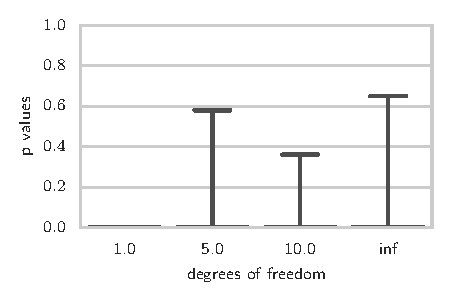
\includegraphics{sgld_student_bad}
\par\end{centering}

\selectlanguage{british}%
\caption{\selectlanguage{english}%
Large autocovariance, unsuitable bootstrap. The parameter $a_{n}$
is too large and the bootstrapped V-statistics $B_{n}$ are, on average,
too low. Therefore it is very likely that $V_{n}>B_{n}$ and the test
is too conservative. \foreignlanguage{british}{\label{fig:student_bad}}\selectlanguage{british}%
}
\end{figure}


\selectlanguage{english}%
In our first task, we modify experiment 4.1 from \citealt{gorham2015measuring}.
The null hypothesis is that the observed samples come from a standard
normal distribution. We study the power of the test against samples
from a Student's t distribution. We expect to observe low p-values
when testing against a Student's t distribution with few degrees of
freedom. We considered 1, 5, 10 or $\infty$ degrees of freedom, where
$\infty$ is equivalent to sampling from a standard normal distribution.
For a fixed number of degrees of freedom we drew 1400 samples and
calculated the p-value. This procedure was repeated one hundred times,
and the bar plots of p-values are shown in Figures \ref{fig:student_bad},\ref{fig:studentst},\ref{fig:thinning}. 

\begin{figure}
\centering{}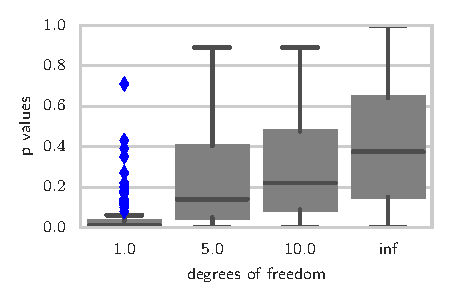
\includegraphics{sgld_student} \caption{Large autocovariance, suitable bootstrap. The parameter $a_{n}$is
chosen suitably, but due to a large autocorrelation withing the samples,
the power of the test is small (effective sample size is small). \label{fig:studentst}}
\end{figure}


\selectlanguage{british}%
The twist on \foreignlanguage{english}{the original experiment 4.1
by \citealt{gorham2015measuring} is that in our case, the draws from
the Student's t distribution were given temporal correlation. The
samples were generated using a Metropolis\textendash Hastings algorithm,
with a Gaussian random walk (variance equal to 0.5). We emphasize
the need for an appropriate choice of the wild bootstrap process parameter,
$a_{n}$, which indicates the probability of a sign flip. In Figure
\ref{fig:student_bad} we plot p-values for $a_{n}$ being set to
$0.5$. Such a high value of $a_{n}$ is suitable for iid observations,
but results in p-values that are too conservative for temporally correlated
observations. In Figure \ref{fig:studentst}, $a_{n}=0.02$, which
gives a well calibrated distribution of the p-values under the null
hypothesis (see box plot for an infinite number degrees of freedom),
however the power of the test is reduced. Indeed, p-values for five
degrees of freedom are already large. The solution that we recommend
is a mixture of thinning and adjusting $a_{n},$ as presented in the
Figure \ref{fig:thinning}. We have thinned the observations by a
factor of 20 and set $a_{n}=0.1$, thus preserving both good statistical
power and correct calibration of p-values under the null hypothesis.}

\begin{figure}
\centering{}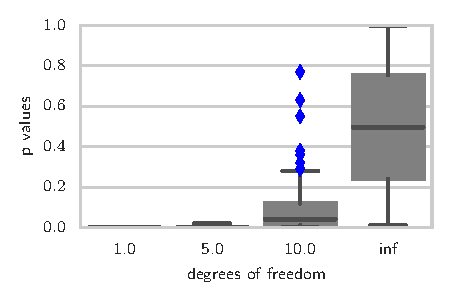
\includegraphics{sgld_student_opt}\caption{\selectlanguage{english}%
Thinned sample, suitable bootstrap. Most of the auto-correlation within
the sample is canceled by thinning. To guarantee that the remaining
autocorrelation is handled properly, the flip probability is set at
$0.1$. \foreignlanguage{british}{\label{fig:thinning}}\selectlanguage{british}%
}
\end{figure}



\subsubsection*{Statistical Model Criticism on Gaussian Processes}

\begin{figure}
\begin{centering}
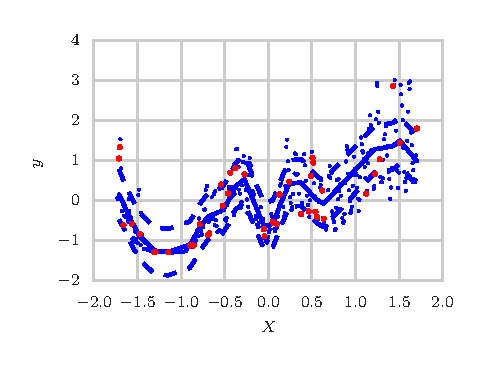
\includegraphics{gp_regression_data_fit}
\par\end{centering}

\caption{Fitted GP and data used to fit (blue) and to apply test (red).\label{fig:experiment_gp_fit}}
\end{figure}


We next apply our test to the problem of statistical model criticism
for GP regression. Our presentation and approach are similar to the
non i.i.d. case of \citet[Section 6]{lloyd2015statistical}. We used
the Solar dataset, consisting of a 1D regression problem with $N=402$
pairs $(X,y)$. We fit $N_{\text{train}}=361$ data using a GP with
a squared exponential kernel and a Gaussian noise model, and performed
standard maximum likelihood II on the hyperparameters (length-scale,
overall scale, noise-variance). We then applied our test to the remaining
$N_{\text{test}}=41$ data. Our test attempts to falsify the null
hypothesis that the Solar dataset was generated from the predictive
distribution (conditioned on training data and predicted position)
of the GP. \citet{lloyd2015statistical} refer to this setup as non
i.i.d., since the predictive distribution is a different univariate
Gaussian for every predicted point. Note that in contrast to their
MMD-based method, our test does \emph{not} need to simulate from the
multiple predictive distributions. Our particular $N_{\text{train}},N_{\text{test}}$
were chosen to make sure the GP fit has stabilised, i.e. adding more
data did not cause further model refinement. Figure \ref{fig:experiment_gp_fit}
shows training and testing data, and the fitted GP. Clearly, the Gaussian
noise model is a poor fit for this particular dataset, e.g. around
$X=-1$. Figure \ref{fig:experiment_gp_test} shows the distribution
over $D=10000$ bootstrapped V-statistics $B_{n}$ with $n=N_{\text{test}}$.
The  test statistic lies in an upper quantile of the bootstrapped
null distribution, indicating (correctly) that it is unlikely the
test points were generated by the fitted GP model, even for the low
number of test data observed, $N_{\text{test}}=41$.

\begin{figure}
\begin{centering}
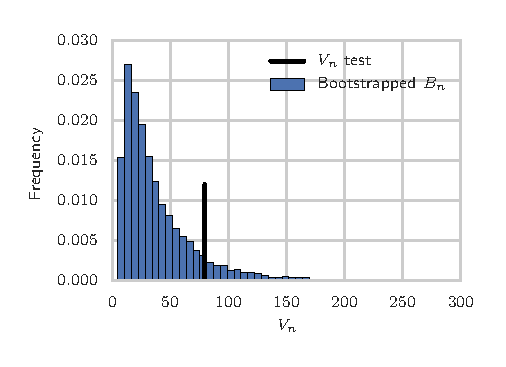
\includegraphics[scale=0.85]{gp_regression_bootstrap_hist}
\par\end{centering}

\caption{Bootstrapped $B_{n}$ distribution with the test statistic $V_{n}$
marked.\label{fig:experiment_gp_test} }
\end{figure}


\selectlanguage{english}%

\subsubsection*{Approximate MCMC algorithm }

\begin{figure}
\centering{}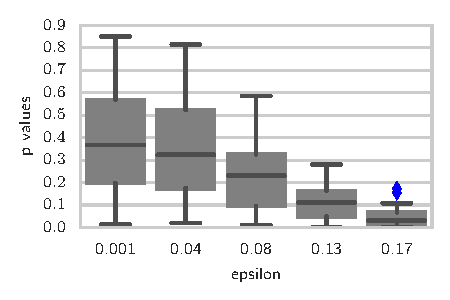
\includegraphics{Heiko1}\foreignlanguage{british}{\caption{\selectlanguage{english}%
Distribution of p-values as a function of $\epsilon$ for austerity
MCMC. \label{p-values}\selectlanguage{british}%
}
}
\end{figure}


We show how to quantify\foreignlanguage{british}{ bias-variance trade-offs
in an approximate }MCMC algorithm\foreignlanguage{british}{ -- }austerity
MCMC \citep{korattikara2013austerity}\foreignlanguage{british}{.
}For the purpose of illustration we use a simple generative model
from \citet{gorham2015measuring,welling2011bayesian}, 
\begin{align*}
\theta_{1}\sim N(0,10);\theta_{2}\sim N(0,1)\\
X_{i}\sim\frac{1}{2}N(\theta_{1},4)+\frac{1}{2}N(\theta_{2},4) & .
\end{align*}
\foreignlanguage{british}{}
\begin{figure}
\centering{}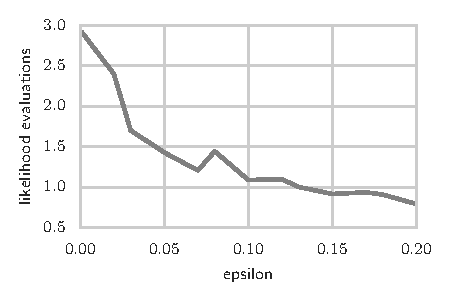
\includegraphics{Heiko2}\foreignlanguage{british}{\caption{\selectlanguage{english}%
Average number of likelihood evaluations a function of $\epsilon$
for austerity MCMC (the y-axis is in millions of evaluations). \label{lik-evals}\selectlanguage{british}%
}
}
\end{figure}
Austerity MCMC is a Monte Carlo procedure designed to reduce the number
of likelihood evaluation in the acceptance step of the Metropolis-Hastings
algorithm. The crux of method is to look at only a subset of the data,
and make an acceptance/rejection decision based on this subset. The
probability of making a wrong decision is proportional to a parameter
$\epsilon\in[0,1]$ . This parameter influences the time complexity
of Austerity MCMC: when $\epsilon$ is larger, i.e., when there is
a greater tolerance for error, the expected computational cost is
lower. We simulated $\{X_{i}\}_{1\leq i\leq400}$ points from the
model with $\theta_{1}=0$ and $\theta_{2}=1$. In this setting there
were two modes in the posterior distribution: one at $(0,1)$ and
the other at $(1,-1)$. We ran the Austerity algorithm with $\epsilon$
varying over the range $[0.001,0.2]$. For each $\epsilon$ we calculated
an individual thinning factor, such that correlation between consecutive
 samples from the chains was smaller than $0.5$ (greater $\epsilon$
generally required more thinning). For each $\epsilon$ we tested
the hypothesis that $\{\theta_{i}\}_{1\leq i\leq500}$ were drawn
from the true stationary posterior, using our goodness of fit test.
We generated 100 p-values for each $\epsilon$ , as shown in Figure
\ref{p-values}. It is clear that $\epsilon=0.09$ yields a good approximation
of the true stationary distribution, while being parsimonious in terms
of likelihood evaluations, as shown in Figure \ref{lik-evals}. 

\selectlanguage{british}%

\subsubsection*{Convergence in non-parametric density estimation}

\begin{figure}
\begin{centering}
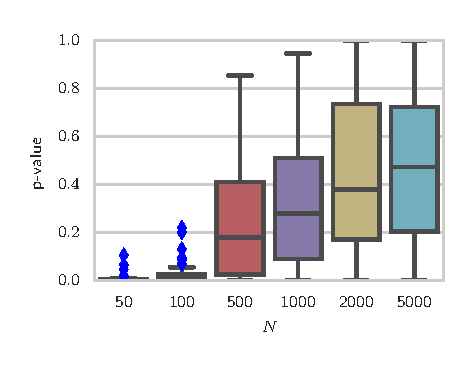
\includegraphics{increasing_data_fixed_test}
\par\end{centering}

\caption{Density estimation: P-values for an increasing number of data $N$
for the non-parametric model.}


\label{fig:density_estimation_increasing_data}
\end{figure}


In our final experiment, we apply our goodness of fit test to measuring
quality-of-fit in nonparametric density estimation. We evaluate two
density models: the infinite dimensional exponential family \citep{SriFukKumGreHyv14},
and a recent approximation to this model using random Fourier features
\citep{strathmann2015gradient}. Our implementation of the model assumes
the log density to take the form $f(x)$, where $f$ lies in an RKHS
induced by a Gaussian kernel with bandwidth $1$. We fit the model
using $N$ observations drawn from a standard Gaussian, and performed
our quadratic time test on a separate evaluation dataset of fixed
size, $N_{\text{test}}=500$. Our goal was to identify $N$ sufficiently
large that the goodness of fit test did not reject the null hypothesis
(i.e., the model had learned the density sufficiently well, bearning
in mind that it is guaranteed to converge for sufficiently large $N$).
Figure \ref{fig:density_estimation_increasing_data} shows how the
distribution of p-values evolves as a function of $N$; this distribution
is uniform for $N=5000$, but at $N=500$, the null hypothesis would
very rarely be rejected.

We next consider the random fourier feature approximation to this
model, where the log pdf, $f$, is approximated using a finite dictionary
of random Fourier features \citep{Rahimi2007}. The natural question
when using this approximation is: ``How many random features do it
I need?'' Using the same test power $N_{\text{test}}=500$ as above,
and a large number of available samples $N=5\cdot10^{4}$, Figure
\ref{fig:density_estimation_increasing_features} shows the distributions
of p-values for an increasing number of random features $m$. From
about $m=50$, the null hypothesis would rarely be rejected, given
a reasonable choice of test level. Note, however, that the p-values
do \emph{not} have a uniform distribution, even for a large number
of random features. This subtle effect is caused by over-smoothing
due to the regularisation approach taken in \citep[KMC finite]{strathmann2015gradient},
which would not otherwise have been detected.  

\begin{figure}
\begin{centering}
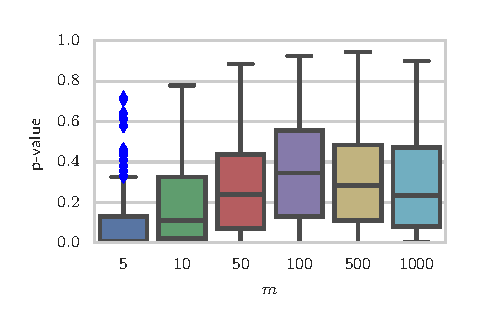
\includegraphics{increasing_features_fixed_test}
\par\end{centering}

\caption{Approximate density estimation: P-values for an increasing number
of random features $m$.}


\label{fig:density_estimation_increasing_features}
\end{figure}


\FloatBarrier

\newpage{}

\bibliographystyle{icml2015}
\bibliography{biblio}


\pagebreak{}

\normalsize\onecolumn


\part*{Appendix}

\selectlanguage{english}%

\section{Proofs}
\begin{lem}
\label{lem:easy} If a random variable $X$ is distributed according
to $p$, then for all $f\in\mathcal{F}$, the expected value of $T$
is zero, i.e. $\ev(Tf)(X)=0$.\end{lem}
\begin{proof}
This result was proved on bounded domains $\mathcal{X}\subset\mathbb{R}^{d}$
by \citet[Lemma 1]{OatGirCho15}, under conditions on the kernel
\begin{align*}
0 & =\oint_{\partial\mathcal{X}}k(x,x')p(x)n(x)dS(x'),\\
0 & =\oint_{\partial\mathcal{X}}\nabla_{x}k(x,x')^{\top}n(x')p(x')dS(x'),
\end{align*}
where $n(x)$ is the unit vector normal to the boundary at $x$, and
$\oint_{\partial\mathcal{X}}$ is the surface integral over the boundary
$\partial\mathcal{X}$. The case of unbounded domains was discussed
by \citet[Remark 2]{OatGirCho15}. Here we provide an alternative,
elementary proof for the latter case. First we show that the functions
$g_{i}=p\cdot f_{i}$ vanish at infinity, by which we mean that for
all dimensions $j$ 
\[
\lim_{x_{j}\to\infty}g_{i}(x_{1},\cdots,x_{d})=0.
\]
The density function $p$ vanishes at infinity. The function $f$
is bounded, which is implied by Cauchy-Schwarz inequality -- $\left|f(x)\right|\le\left\Vert f\right\Vert \sqrt{k(x,x)}$.
This implies that the function $g$ vanishes at infinity. To show
the expected value $\ev(T_{p})f(X)$ is zero, it is sufficient to
show that for all dimensions $i$, the expected value of $\frac{\partial\log p(X)}{\partial x_{i}}f_{i}(X)+\frac{\partial f_{i}(X)}{\partial x_{i}}$
is zero. 
\begin{align*}
 & \ev\left(\frac{\partial\log p(x)}{\partial x_{i}}f_{i}(x)+\frac{\partial f_{i}(x)}{\partial x_{i}}\right)\\
 & =\int_{R_{d}}\left[\frac{\partial\log p(x)}{\partial x_{i}}f_{i}(x)+\frac{\partial f_{i}(x)}{\partial x_{i}}\right]q(x)dx\\
 & =\int_{R_{d}}\left[\frac{1}{p(x)}\frac{\partial q(x)}{\partial x_{i}}f(x)+\frac{\partial f(x)}{\partial x_{i}}\right]q(x)dx\\
 & =\int_{R_{d}}\left[\frac{\partial p(x)}{\partial x_{i}}f_{i}(x)+\frac{\partial f_{i}(x)}{\partial x_{i}}q(x)\right]dx\\
 & \overset{(a)}{=}\int_{R_{d-1}}\left(\lim_{R\to\infty}p(x)f_{i}(x)\bigg|_{x_{i}=-R}^{x_{i}=R}\right)dx_{1}\cdots dx_{i-1}\cdots dx_{i+1}\cdots d{x_{d}}\\
 & =\int_{R_{d-1}}0dx_{1}\cdots dx_{i-1}\cdots dx_{i+1}\cdots d{x_{d}}\\
 & =0.
\end{align*}
For the equation (a) we have used integration by parts, fact that
$g_{i}$ vanishes at infinity and Fubini-Toneli theorem to show that
we can do iterated integration. The sufficient condition for the Fubini-Toneli
theorem is that $\int|g_{i}f(x)|q(x)dx$ exists. This is implied by
existence of $\ev|\frac{\partial\log p(X)}{\partial x_{i}}f_{i}(X)|$
and $\ev|\frac{\partial f_{i}(X)}{\partial x_{i}}|$. Since $f_{i}$
is bounded and $\ev|\frac{\partial\log p(X)}{\partial x_{i}}|\leq\ev\|\nabla\log p(Z)\|^{2}$,
condition ii) guarantees that $\ev|\frac{\partial\log p(X)}{\partial x_{i}}f_{i}(X)|$
is finite. For the second term we have $\ev|\frac{\partial f_{i}(X)}{\partial x_{i}}|=\ev|\langle\frac{\partial k(X,cdot)}{\partial x_{i}},f_{i}|\rangle\leq\|f_{i}\|_{\mathcal{F}}\ev\sqrt{\frac{\partial^{2}k(X,X)}{dx_{i}dx_{i+d}}}$,
which is guaranteed by the condition iv). 
\end{proof}
\selectlanguage{british}%

\selectlanguage{english}%
\begin{proof}[Proof of \foreignlanguage{british}{proposition} \ref{thm: null_dist}]
We check assumptions of the Theorem 2.1 \citep{leucht2012degenerate}.
The condition A1, $\sum_{t=1}^{\infty}\sqrt{\tau(t)}\leq\infty$,
is implied by assumption $\sum_{t=1}^{\infty}t^{2}\sqrt{\tau(t)}\leq\infty$
in Section \ref{sec:Details}. Condition A2 (iv), Lipschitz continuity
of $h$, follows from assumption (iv). Conditions A2 i), ii) positive
definiteness, symmetry and degeneracy of $h$ follow from the proof
of Theorem (\ref{theorem_discrepancy_is_metric}). Indeed

\[
h(x,y)=\langle\left[\nabla\log p(x)k(x,\cdot)+\nabla_{1}k(x,\cdot)\right],\left[\nabla\log p(y)k(y,\cdot)+\nabla_{1}k(y,\cdot)\right]\rangle_{\mathcal{F}^{d}}
\]
\\
so the statistic is an inner product and hence positive definite.
Degeneracy under the null follows from the fact that for any $t$,
by Lemma (\ref{lem:easy}),$\ev(\nabla\log p(x)k(x,t)+\nabla_{1}k(x,t))=0$.
Finally, condition A2 (iii), $\ev h(X,X)\leq\infty$ follows from
assumptions (ii), (iii) and boundedness of the kernel.
\end{proof}
\selectlanguage{british}%

\selectlanguage{english}%
\begin{proof}[Proof of \foreignlanguage{british}{proposition \ref{thm:wild_bootstrap_works}}]
We use Theorem 2.1 \citep{leucht2012degenerate} to see that, under
the null hypothesis, $f(W_{1,n},\cdots,W_{t,n})$ converges to zero
in probability. We have checked assumptions A1,A2 in the proof of
the proposition \foreignlanguage{british}{\ref{thm: null_dist}}.
Assumption B1 is identical to our assumption from Section \ref{sec:Details}
. Finally we check assumption B2 (bootstrap assumption):\emph{ $\{W_{t,n}\}_{1\leq t\leq n}$}
is a row-wise strictly stationary triangular array independent of
all $Z_{t}$ such that $\ev W_{t,n}=0$ and $\sup_{n}\ev|W_{t,n}^{2+\sigma}|=1<\infty$
for some $\sigma>0$. The auto-covariance of the process is given
by $\ev W_{s,n}W_{t,n}=(1-2p_{n})^{-|s-t|}$, so the function $\rho(x)=\exp(-x)$,
and $l_{n}=\log(1-2p_{n})^{-1}$. We verify that $\lim_{u\to0}\rho(u)=1$.
If we set $p_{n}=w_{n}^{-1}$ , such that $w_{n}=o(n)$ and $\lim_{n\to\infty}w_{n}=\infty$,
then $l_{n}=O(w_{n})$ and $\sum_{r=1}^{n-1}\rho(|r|/l_{n})=\frac{1-(1-2p_{n})^{n+1}}{p_{n}}=O(w_{n})=O(l_{n})$.
Finally we show that $B_{n}$ converges to zero under the alternative.
It is sufficient to check that $\ev B_{n}\to0,\ev B_{n}^{2}\to0.$

\begin{align*}
\ev B_{n} & =\frac{1}{n^{2}}\sum_{i,j}\ev W_{i}W_{j}\ev h(Z_{i},Z_{j})\\
 & =\frac{1}{n^{2}}\sum_{i\in N^{m}}\rho(|j-i|/l_{n})\ev h(Z_{j},Z_{i})\\
 & \leq\frac{1}{n^{2}}\sum_{i\in N^{m}}\rho(|j-i|/l_{n})C\\
 & \to0
\end{align*}
\foreignlanguage{british}{for some constant $C=\ev h(Z_{1},Z_{2})$,
whose existence follows from assumptions i) and iii). As for $\ev B_{n}^{2}$,
we have}

\begin{align*}
\ev B_{n}^{2} & =\frac{1}{n^{4}}\sum_{i,j,k,l}\ev W_{i}W_{j}W_{k}W_{l}\ev h(Z_{i},Z_{j})h(Z_{k},Z_{l})\\
 & \leq\frac{1}{n^{4}}\sum_{i\neq j,i\neq k,i\neq l,j\neq k,j\neq l,k\neq l}\ev W_{i}W_{j}W_{k}W_{l}\ev h(Z_{i},Z_{j})^{2}\ev h(Z_{k},Z_{l})^{2}+C'\frac{6n^{3}}{n^{4}}\\
 & \leq\frac{1}{n^{4}}\sum_{i\neq j,i\neq k,i\neq l,j\neq k,j\neq l,k\neq l}\ev W_{i}W_{j}W_{k}W_{l}C'+\frac{6C'}{n}\\
 & =\frac{6C'}{n}\to0,
\end{align*}
\foreignlanguage{british}{where $C'=\ev h(Z_{i},Z_{j})^{2}\ev h(Z_{k},Z_{l})^{2}$.}
\end{proof}

\subsection{Linear time test }

We may use similar reasoning for the quadratic time test to define
a linear time test, based on the two-sample test of \citet{Chwialkowski2015}.
For some fixed location $y$ and a random variable $X$, define a
random variable $s(X,y)$ as 
\begin{align}
s(X,y)=\nabla\log p(X)g(X,y)-\nabla g(X,y).
\end{align}
For some number of random locations $Y_{1},Y_{J}$ and a random variable
$X$ define a random vector $Z_{i}$ 
\begin{equation}
Z_{i}=(s(X_{i},Y_{1}),\cdots,s(X_{i},Y_{J}))\in\mathbf{R}^{J}.
\end{equation}
Let $W_{n}$ be a mean of $Z_{i}$'s $W_{n}=\frac{1}{n}\sum_{i=1}^{n}Z_{i},$
and $\Sigma_{n}$ its covariance matrix $\Sigma_{n}=\frac{1}{n}ZZ^{T}$.
The test statistic is 
\begin{equation}
S_{n}=nW_{n}\Sigma_{n}^{-1}W_{n}.
\end{equation}
The computation of $S_{n}$ requires inversion of a $J\times J$ matrix
$\Sigma_{n}$, but this is fast and numerically stable: $J$ will
typically be small, and is less than 10 in our experiments. The next
proposition demonstrates the use of $S_{n}$ as a one-sample test.
\begin{prop}[Asymptotic behavior of $S_{n}$]
 \label{prop:Hotelling} If $\ev s(X,y)=0$ for all $y$, then the
statistic $S_{n}$ is a.s. asymptotically distributed as a $\chi^{2}$-random
variable with $Jd$ degrees of freedom, where $d$ is $X$ dimensionality
(as $n\to\infty$ with $d$ fixed). If $\ev s(X,y)\neq0$ for almost
all $y$ then a.s. for any fixed $r$, $\mathbb{P}(S_{n}>r)\to1$
as $n\to\infty$ . 
\end{prop}

\paragraph{One sample test}

Calculate $S_{n}$. Choose a threshold $r_{\alpha}$ corresponding
to the $1-\alpha$ quantile of a $\chi^{2}$ distribution with $J$
degrees of freedom, and reject the null hypothesis whenever $S_{n}$
is larger than $r_{\alpha}$. \selectlanguage{british}%

\end{document}
